\documentclass{article}
\usepackage{amsmath}
\usepackage{amsfonts}
\usepackage[english]{babel}
\usepackage[utf8]{inputenc}
\usepackage{amsthm}
\usepackage{graphicx}

\newcommand{\norm}[1]{\left\lVert#1\right\rVert}
\newtheorem{theorem}{Theorem}
\newtheorem{prop}{Proposition}
\newcommand{\overbar}[1]{\mkern 1.5mu\overline{\mkern-1.5mu#1\mkern-1.5mu}\mkern 1.5mu}

\begin{document}

\title{Homework 5}
\author{Toby Harvey}
\maketitle

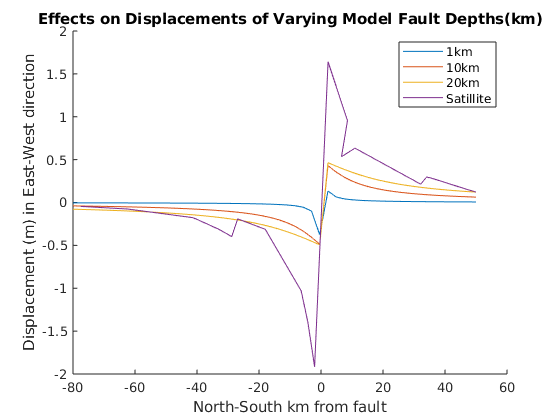
\includegraphics[width=\linewidth]{fault_depth.png}

As the fault gets deeper the displacements in the east-west direction farther from the fault, in the north-south direction, grow. i.e. Fault depth effects the amount of displacement away from the fault, more than near the fault.

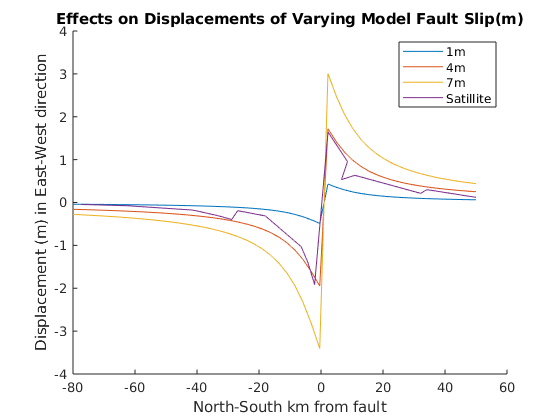
\includegraphics[width=\linewidth]{fault_slip.png}

As slip increases, displacements near the fault grow faster than  displacements far from the fault. 

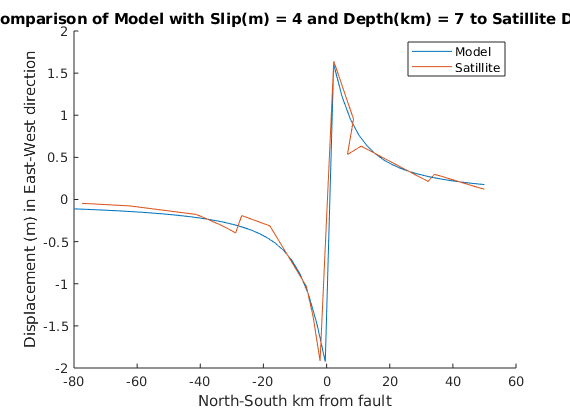
\includegraphics[width=\linewidth]{opt_fault.png}

\newpage

\noindent Possible reasons why the model doesn't perfectly fit the Satillite data:

\noindent *We are assuming isotropic media in our model (i.e. when we use Hookes law to derive our model we are assuming that $\lambda$ and $\mu$ are constant in space)


\noindent *There is error in the Satillite measurements.





\end{document}
